\documentclass[12pt]{article}
\setlength{\oddsidemargin}{0in}
\setlength{\evensidemargin}{0in}
\setlength{\textwidth}{6.5in}
\setlength{\parindent}{0in}
\setlength{\parskip}{\baselineskip}

\usepackage[utf8]{inputenc}
\usepackage{amsmath,amsfonts,amssymb,graphicx, qtree}

\title{Peterson-Ian-0320-PS4}
\author{Ian Peterson}
\date{May  31, 2019}

\begin{document}

CSCI 3104 Summer 2019 \hfill  Problem Set 4\\
Ian Peterson (03/20)\hfill Ian.Peterson@Colorado.edu

\hrulefill\\
Compiled with \LaTeX

\begin{enumerate}
    
    \item \textit{Problem 1}

    Shadow is writing a secret message to Harry and wants to prevent it from being understood by Thormund. He decides to use Huffman encoding to encode the message. Magically, the symbol frequencies of the message are given by the Lucas numbers, a famous sequence of integers discovered by the same person who discovered the Fibonacci numbers. The nth Lucas number is defined as $L_n = L_{n-1} + L_{n-2}$ for $n > 1$ with base cases $L_0$ = 2 and $L_1$ = 1.\\
    
    \begin{enumerate}
        \item 
        
        \label{q:huff:a} For an alphabet of $\Sigma=\{a,b,c,d,e,f,g,h\}$ with frequencies given by the first $|\Sigma|$ Lucas numbers, give an optimal Huffman code and the corresponding encoding tree for Shadow to use.\\
        
        Answer:\\
    
        By using Huffman Coding we find the following frequencies:\\
    \begin{center}
    	\begin{tabular}{|c|c|c|c|c|c|c|c|}
    		\hline
    		a & b & c & d & e & f & g & h\\
    		\hline
    		2 & 1 & 3 & 4 & 7 & 11 & 18 & 29\\
    		\hline
    	\end{tabular}
    \end{center}
    
        This leads us to constructing the tree by making a min heap, and combining the smallest two elements until we have our root node being the sum of the given frequencies.\\
        
        \Tree[.75 [.h
        ]
                [.46 [.g
                ]
                    [.28 [.f
                    ]
                           [.17 [.e
                           ]
                                [.10 [.d
                                ]
                                    [.6 [.c
                                    ]
                                        [.3 [.b
                                        ]
                                            [.a
                                            ]]]]]]]]\\
        
        Given that in the path each left subtree is a 0 in code form, and each right subtree is a 1, we finally determine the Huffman code for this example to be as follows for each letter in the alphabet:\\
        
    \begin{center}
    	\begin{tabular}{|c|c|}
    		\hline
    		a & 1111111\\
    		\hline
    		b & 1111110\\
    		\hline
    		c & 111110\\
    		\hline
    		d & 11110\\
    		\hline
    		e & 1110\\
    		\hline
    		f & 110\\
    		\hline
    		g & 10\\
    		\hline
    		h & 0\\
    		\hline
    	\end{tabular}
    \end{center}
        
        \item 
        
        Generalize your answer to (\ref{q:huff:a}) and give the structure of an optimal code when the frequencies are the first $n$ Lucas numbers.\\
        
        Answer:\\
    
        In the first part of the question our n was 8 given 8 letters in our alphabet. This number correspoinded to the levels in our tree. For a Huffman code of length n, we expect the code to have the first letter correspond with n-1 1s, followed by n-2 1s, and a zero, followed by n-3 1s and a zero, all the way until we get to the nth letter, and have just a 0. This can be shown as follows in the table.\\
        
        \begin{center}
    	\begin{tabular}{|c|c|}
    		\hline
    		0 & 11111...1\\
    		\hline
    		1 & 11111...10\\
    		\hline
    		2 & 1111...10\\
    		\hline
    		3 & 111...10\\
    		\hline
    		... & ...\\
    		\hline
    		... & ...\\
    		\hline
    		n-1 & 10\\
    		\hline
    		n & 0\\
    		\hline
    	\end{tabular}
    \end{center}
        
    \end{enumerate}
    
    \newpage

    \item \textit{Problem 2}

    A good hash function $h(x)$ behaves in practice very close to the uniform hashing assumption analyzed in class, but is a deterministic function. That is, $h(x)=k$ each time $x$ is used as an argument to $h()$. Designing good hash functions is hard, and a bad hash function can cause a hash table to quickly exit the sparse loading regime by overloading some buckets and under loading others. Good hash functions often rely on beautiful and complicated insights from number theory, and have deep connections to pseudorandom number generators and cryptographic functions. In practice, most hash functions are moderate to poor approximations of uniform hashing.
	
	\smallskip Consider the following hash function. Let $U$ be the universe of strings composed of the characters from the alphabet $\Sigma=[${\tt A}$,\dots,${\tt Z}$]$, and let the function $f(x_{i})$ return the index of a letter $x_{i}\in \Sigma$, e.g., $f(${\tt A}$)=1$ and $f(${\tt Z}$)=26$. Finally, for an $m$-character string $x\in \Sigma^{m}$, define $h(x) = \left(\left[\sum_{i=1}^{m}f(x_{i})\right]\!\! \mod \ell\right)$, where $\ell$ is the number of buckets in the hash table. That is, our hash function sums up the index values of the characters of a string $x$ and maps that value onto one of the $\ell$ buckets.\\
    
    \begin{enumerate}
        \item 
        
        The following list contains US Census derived last names: \\
    	{\tt http://www2.census.gov/topics/genealogy/1990surnames/dist.all.last} \\
    	Using these names as input strings, first choose a uniformly random 50\% of these name strings and then hash them using $h(x)$.
    	
    	Produce a histogram showing the corresponding distribution of hash locations when $\ell=200$. Label the axes of your figure. Briefly describe what the figure shows about $h(x)$, and justify your results in terms of the behavior of $h(x)$. Do not forget to append your code.
    	 
    	{\footnotesize Hint: the raw file includes information other than name strings, which will need to be removed; and, think about how you can count hash locations without building or using a real hash table.}\\
        
        Answer:\\
    
        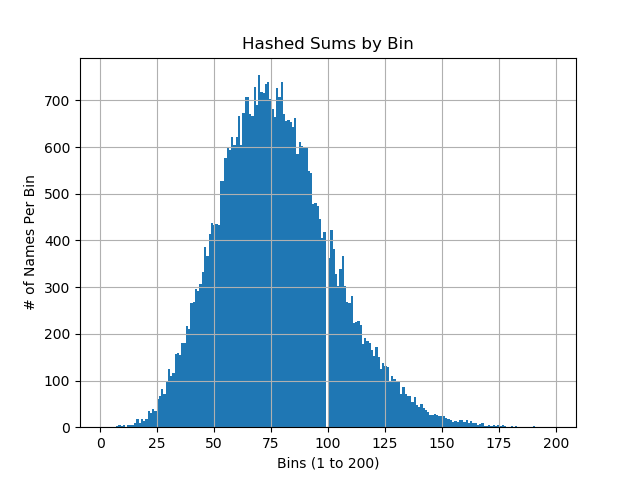
\includegraphics[width=6in]{PS4FIG1.png}\newline
        The above figure shows that given our current implementation of the hash function $h(x)$, our hashing is not uniform, but rather resembles a bell curve of some sort. Because our collisions are not evenly distributed among all 200 bins, the hash is not efficient and the time complexity gets very bad as compared to how it might be with a more uniform hash. We could have expected this as most of the name sums don't even pass 200, so the hashing function does little to evenly distribute, and the curve we see in the histogram above seems as though it would also accurately portray the names when summed by index in the alphabet.(Code included in submission.)\\
        
        \item 
        
        Enumerate at least 4 reasons why $h(x)$ is a bad hash function relative to the ideal behavior of uniform hashing.\\
        
        Answer:\\
        
        \begin{enumerate}
            \item 
            
            It does not have an effect on a majority of values as the modulus function does nothing to change values under the number 200 in our case, which encompasses all of our results as far as one can tell with the data set presented.\\
            
            \item
            
            The curve present in an ideal hashing function would be a straight line showing all buckets are being used properly to resolve and minimize collisions, but ours is a large curve with some of the buckets appearing to not be used at all.\\
            
            \item
            
            The longest chains in this hash table account for a significant portion of the total data set, meaning that if one were to search or perform other operations, the time complexity in the worst case approaches that of a linked list, which for such large data sets is far too slow.\\
            
            \item
            
            Again, with the number of data points present, even the shortest chains are really long, so most results of this hash will provide collisions, and thus the efficiency of the program is reduced because collision resolution is almost a requirement for most of the insertions that occur.\\
            
        \end{enumerate}\\
        
        \item 
        
        Produce a plot showing (i) the length of the longest chain (were we to use chaining for resolving collisions under $h(x)$) as a function of the number $n$ of these strings that we hash into a table with $\ell=200$ buckets, (ii) the exact upper bound on the depth of a red-black tree with $n$ items stored, and (iii) the length of the longest chain were we to use a uniform hash instead of $h(x)$. Include a guide of $c\,n$
    	
    	Then, comment (i) on how much shorter the longest chain would be under a uniform hash than under $h(x)$, and (ii) on the value of $n$ at which the red-black tree becomes a more efficient data structure than $h(x)$ and separately a uniform hash.\\
        
        Answer:\\
    
        Plots:\\
        \begin{enumerate}
            \item 
            \\
            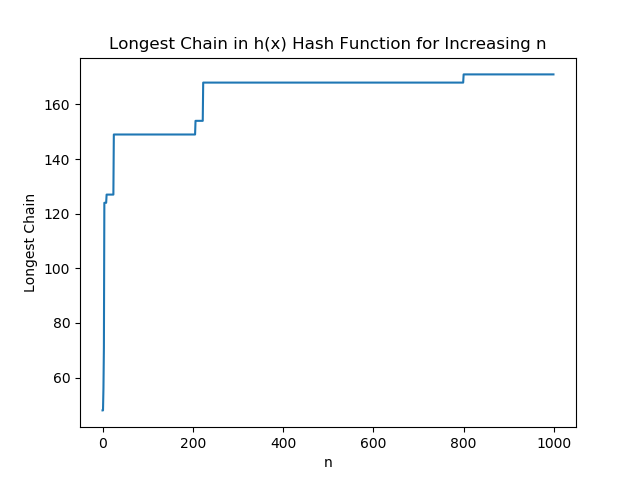
\includegraphics[width=6in]{PS4FIG2.png}\newline
            \\
            \item
            \\
            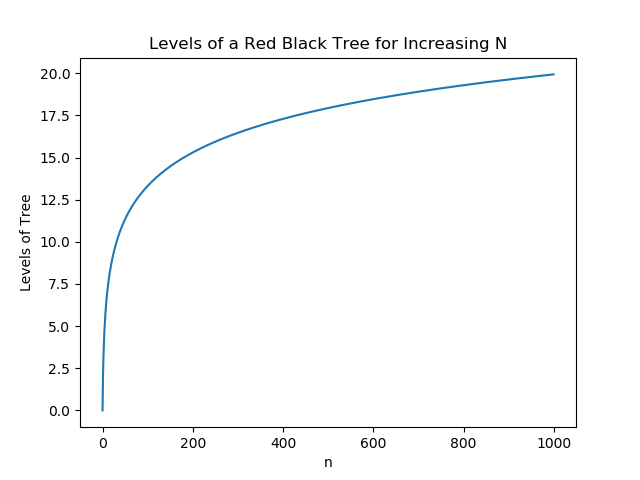
\includegraphics[width=6in]{PS4FIG3.png}\newline
            \\
            \item
            \\
            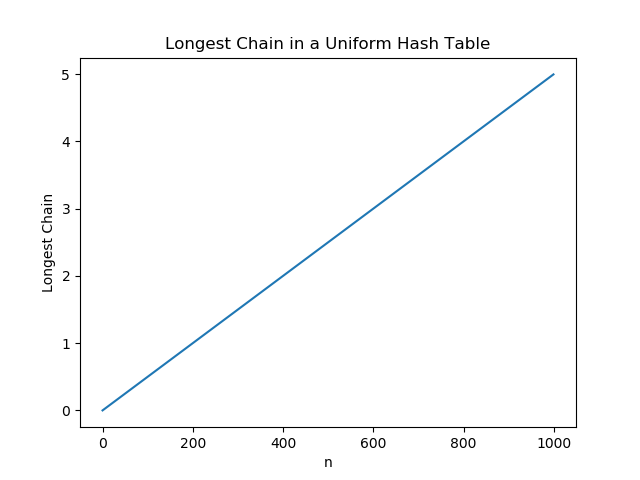
\includegraphics[width=6in]{PS4FIG4.png}\newline
            \\
        \end{enumerate}
        Comments:\\
        \begin{enumerate}
            \item 
            
            The uniform hash is much smaller than our h(x) hash as the uniform hash's longest chain is only ever $\frac{n}{200}$ long, and the h(x) is consistently much larger.\\
            
            \item
            
            A uniform hash is almost always better because it has less collisions and thus has shorter chains at all times. The red black tree on the other hand although much worse than the uniform hash, it is still almost always better than the h(x) hash for values larger than about 50. The h(x) hash has so many collisions in just the first 100 values that on a larger scale it is always better, but for perhaps the first 20-40 elements, it is possible that the h(x) hash will be better than a red black tree.\\
            
        \end{enumerate}
        
    \end{enumerate}
    
    \newpage

    \item \textit{Problem 3}
    
    Grog is struggling with the problem of making change for $n$ cents using the smallest number of coins for his purchase of a new great sword. Grog has coin values of $v_{1}<v_{2}<\dots<v_{r}$ for $r$ coin types, where each coin's value $v_{i}$ is a positive integer. His goal is to obtain a set of counts $\{d_{i}\}$, one for each coin type, such that $\sum_{i=1}^{r}d_{i}=k$ and where $k$ is minimized.\\
    
    \begin{enumerate}
        \item 
        
        A greedy algorithm for making change is the \textbf{cashier's algorithm}, which all young wizards learn. Harry writes the following pseudocode on the whiteboard to illustrate it, where $n$ is the amount of money to make change for and $v$ is a vector of the coin denominations:
	%
	\begin{small}
	\begin{verbatim}
	wizardChange(n,v,r) :
	   d[1 .. r] = 0       // initial histogram of coin types in solution
	   while n > 0 {
	      k = 1
	      while ( k < r and v[k] > n ) { k++ }
	      if k==r { return 'no solution' }
	      else { n = n - v[k] }
	   }
	   return d
	\end{verbatim}
	\end{small}
	Thormund snorts and says Harry's code has bugs. Identify the bugs and explain why each would cause the algorithm to fail.\\
        
        Answer:\\
    
        To begin, in the while loop, we are starting with the smallest denomination of money, so our algorithm will always return numbers much too large, as it would simply be using the smallest currency each time. Next, k should be initialized to r as the reasons i previously mentioned, and furthermore, the check in the while condition should instead check that k is larger than 1(assuming the vector indexes from 1 and not 0), as this indicates that we have started with the largest denomination, and come all the way to the smallest in the vector. The very first line has us setting an array to equal 0, when instead we should be setting each index in the array to 0, because if you tried this in most languages, you would get an error back. in the first while loop, where we check that n is larger than 0, we should instead check that n is not equal to zero, because if we go below, then we have messed up calculations elsewhere, and if we made perfect change, we would be stuck as our value never goes negative, so we never leave the loop. Finally the logic in the if else makes no sense, as k should be the iterator going through the denominations, but we state that if we hit our largest denomination, we have no solution which simply makes no sense, however the logic in the else is salvageable if we rewrite the rest, as this is the correct way which we want to decrease n when our denomination fits in the value we are giving change for. Altogether the code is logically incorrect and cannot produce coherent results.\\
        
        \item 
        
        Sometimes the dwarves at Rocky Mountain Bank run out of coins,%
	%
	\footnote{It's a little known secret, but dwarven pets like to \textit{eat} the coins. It isn't pretty for the coins, in the end.}
	%
	and make change using whatever is left on hand. Identify a set of U.S. coin denominations for which the greedy algorithm does not yield an optimal solution. Justify your answer in terms of optimal substructure and the greedy-choice property. (The set should include a penny so that there is a solution for every value of $n$.)
	
%	1. Greedy-choice property: A global optimum can be arrived at by selecting a local optimum.
%	2. Optimal substructure: An optimal solution to the problem contains an optimal solution to subproblems.\\
        
        Answer:\\
    
        With only quarters, dimes, and pennies left, if asked to give change for 30 cents, the greedy algorithm would give a quarter, and five pennies, for a total of six coins while the actual optimal solution would be to give three dimes for a total of three coins. Greedy Choice Property states a global optimum can be arrived at by selecting a local optimum. According to the greedy algorithm, by making the best choice given a current situation, such as finding a coin as close to thirty as possible, it then states it will come to an optimal solution, but as we saw this isn't always the case. When then considering the definition of optimal substructure, we know an optimal solution to the problem contains an optimal solution to sub problems. By finding the minimum coins of the scenario where we use a quarter and the one where we don't we would have then solved sub problems, and found that the better solution would be not taking the quarter, but rather the three dimes result in less overall coins.\\
        
        \item 
        
        On the advice of wizards specializing in electricity, Rocky Mountain Bank has announced that they will be changing all  coin denominations into a new set of coins denominated in powers of $c$, i.e., denominations of $c^{0}, c^{1}, \dots , c^{\ell}$ for some integers $c>1$ and $\ell\geq 1$.  (This will be done by a spell that will magically transmute old coins into new coins, before your very eyes.) Prove that the cashier's algorithm will always yield an optimal solution in this case.
	
	Hint: first consider the special case of $c=2$.\\
        
        Answer:\\
    
        In the above situation, we know that the new coins will be in denominations of $ c^{l} $ where $ c > 1$, and $l \geq 1$ if we assume some value a is the optimal solution to the problem asking what the optimal number of coins to give is for some amount n. To prove that the greedy solution or the cashier's algorithm produces optimal solutions to this problem, we can do a proof by contradiction.\\
        Of course we must first assume the contrapositive, being that any any non-greedy solution is optimal. As above we will assume that $l \geq 1$ & $c > 1$ so considering a non-greedy solution, where $a_{l}$ is the number of coins of denomination $c^{l}$ used in the optimal solution, we can claim $\sum_{l=0}^{i-1}a_{l}*c^l = n$ where i is the maximum value l might reach as a denomination in this scenario. $n$ of course is the value we are making change for, and granted we have to use at least one coin to make the change, we can furthermore make the assertion that $ n \geq c^i $ so it follows by simple substitution that $ \sum_{l=0}^{i-1}a_{l}*c^l \geq c^i $. Under our assumption that this non greedy solution is optimal, we can go on to say that our value $a_{l}$ being the optimal solution for denomination $c^l$ where $l$ is some integer from 0 to t. It follows that for $ l = 0, 1, 2, ..., t-1 $ we can claim $a_{l} < c$. This lets us claim with our summation that $ \sum_{l=0}^{i-1}a_{l}*c^l \leq \sum_{l=0}^{i-1}(c-1)*c^l $, and the right side of that equation can have the constant multiplier pulled outside the summation, and give us $ (c-1)\frac{c^i-1}{c-1} $ which again simplifies to $ c^i - 1 $, and we know that $c^i > c^i-1$, so by one last substitution, we can finally say that $ \sum_{l=0}^{i-1}a_{l}*c^l < c^i $ but this contradicts our original claim, meaning a greedy algorithm must provide the optimal solution.\\
        
    \end{enumerate}
    
    \newpage

    \item \textit{Problem 4}
    
    We saw in the previous problem that the cashier's (greedy) algorithm for making change doesn't handle arbitrary denominations optimally. In this problem you'll develop a dynamic programming solution which does, but with a slight twist. Suppose we have at our disposal an arbitrary number of \emph{cursed} coins of each denomination $d_1, d_2, \dotsc, d_k$, with $d_1 < d_2 < \dotsc < d_k$, and we need to provide $n$ cents in change. We will always have $d_1=1$, so that we are assured we can make change for any value of $n$. The curse on the coins is that in any one exchange between people, with the exception of $i=2$, if coins of denomination $d_i$ are used, then coins of denomination $d_{i-1}$ \emph{cannot} be used. Our goal is to make change using the minimal number of these cursed coins (in a single exchange, i.e., the curse applies).\\
    
    \begin{enumerate}
        \item 
        
        For $i \in \{1,\dotsc,k\}$, $n \in \mathbb{N}$, and $b \in \{0,1\}$, let $C(i,n,b)$ denote the number of cursed coins needed to make $n$ cents in change using only the first $i$ denominations $d_1, d_2, \dotsc, d_i$, where $d_{i-1}$ is allowed to be used if and only if $i \leq 2$ or $b=0$. That is, $b$ is a Boolean ``flag'' variable indicating whether we are excluding denomination $d_{i-1}$ or not ($b=1$ means exclude it). 	
    	Write down a recurrence relation for $C$ and prove it is correct. Be sure to include the base case.\\
        
        Answer:\\
    
        The recurrence relation that applies in this problem is -\\
        $$C(i,n,b) =  \begin{cases} 
            C(i-1,n,0) & b = 1, i > 2 \\
            return & n = 0\\
            return + n & i = 1\\
            C(i-1,n,0) & n < d_{i}\\
            min(C(i-2,n-(d_{i}* \lfloor \frac{n}{d_{}i} \rfloor),0) + \lfloor \frac{n}{d_{}i} \rfloor, C(i-1,n,0)) & otherwise  
            \end{cases}$$
        Proof of by Strong Induction:\\
        First, our base cases are when $n = 0$, for which we have properly made change equalling the value we wished to reach. Our other one is $i=1$, for which we would simply add n to the coins we have thus far collected because our only remaining denomination to consider is 1, so there n=must be n many 1s.\\
        The inductive hypothesis is that this function works for some i of k, so that our solution is optimal.\\
        Our inductive step (i and n) is then to consider that we assume all values less than n are optimal. We can encounter three situations.\\
        \begin{enumerate}
            \item The case where our b flag is 1, and our i counter is still greater than 2, for which we cannot take the current denomination as it is cursed, so we would recurse on the index right before, and toggle the b, flag, meaning we have simply handled a case that problem parameters specify.
            \item The next case we handle is when our denomination is too large to fit within n, so we increment i down one, and maintain our value for n, as well as ensuring our b value is set to 0.
            \item Finally, in the case where we can take the value, in our dynamic programming solution we take the minimum of the scenario in which we take it and the situation in which we do not. In the case we do take it, we must remember we can take multiple coins of the same denomination, so we use the floor function to find whether or not we can take multiple and if so how many, and of course we add the number of coins we then took to our solution. We then decrements by two, as we know we cannot take the next coin denomination due to the curse inflicting them, so we skip the next term and keep b at 0, as we have dealt with the curse manually by decrementing by two. Finally we subtract our denomination multiplied with the amount of the coin we took from n to find our new value of n that the next recurrence must consider. However in the case where we do not take the coin of the current i denomination, we just decrement by one as we did not take it, and keep n and b at their current values.\\
        \end{enumerate}
        
        \item 
        
        Based on your recurrence relation, describe the order in which a dynamic programming table for $C(i,n,b)$ should be filled in.\\
        
        Answer:\\
    
        We can start with our base cases filling in the leftmost and top most column and row, and because the recurrence relies on these cases, we would fill it in from the top left most position to the bottom right, by rows or by columns, wither should work.\\
        
        \item 
        
        Based on your description in part (b), write down pseudocode for a dynamic programming solution to this problem, and give a $\Theta$ bound on its running time (remember, this requires proving both an upper \emph{and} a lower bound).\\
        
        Answer:\\
    
        Pseudocode:\\
        \begin{verbatim}
    OptimalSol(I,n,b){ // I is an array containing the denominations
        M=[][]
        for i = 0 to len(i)
            for n = 0 to n
                if n = 0
                    M[i][n] = 0
                elif i = 1 // I indexes from 1, rather than 0 for 
                                legibility sake
                    M[i][n] = n
                elif n < I[i]
                    M[i][n] = M[i-1][n]
                else
                    M[i][n] = min(M[i-2][n-(I[i]*floor(n/I[i]))] +
                    floor(n/I[i]),M[i-1][n])
        return M[len(i)][n]
    }
        \end{verbatim}\\
        
        Bounded by $\Theta(n^2)$\\
        Proof:\\
        Very rudimentary, as regardless of the values, we will loop through n values n times, to populate the array, and to find the result and perform all calculations it takes constant time, so we have a tight bound on the time complexity.\\
        %Upper and Lower bounds
        
    \end{enumerate}

\end{enumerate}

\end{document}